\documentclass[11pt]{article}
\usepackage[margin=2cm]{geometry}
\usepackage{graphicx}
\usepackage{amsmath,amssymb}
\usepackage{caption}
\usepackage{subcaption}
\usepackage{hyperref}
\usepackage{placeins}

\title{Rebuttal Figures --- Additional Experiments}
\author{}
\date{}

\begin{document}
\maketitle

%% ============================================================
%% SECTION 1: BERT (dense attention) experiments
%% ============================================================

\section{BERT experiments (dense attention)}

\begin{figure}[htbp]
\centering
\begin{subfigure}[b]{0.48\textwidth}
    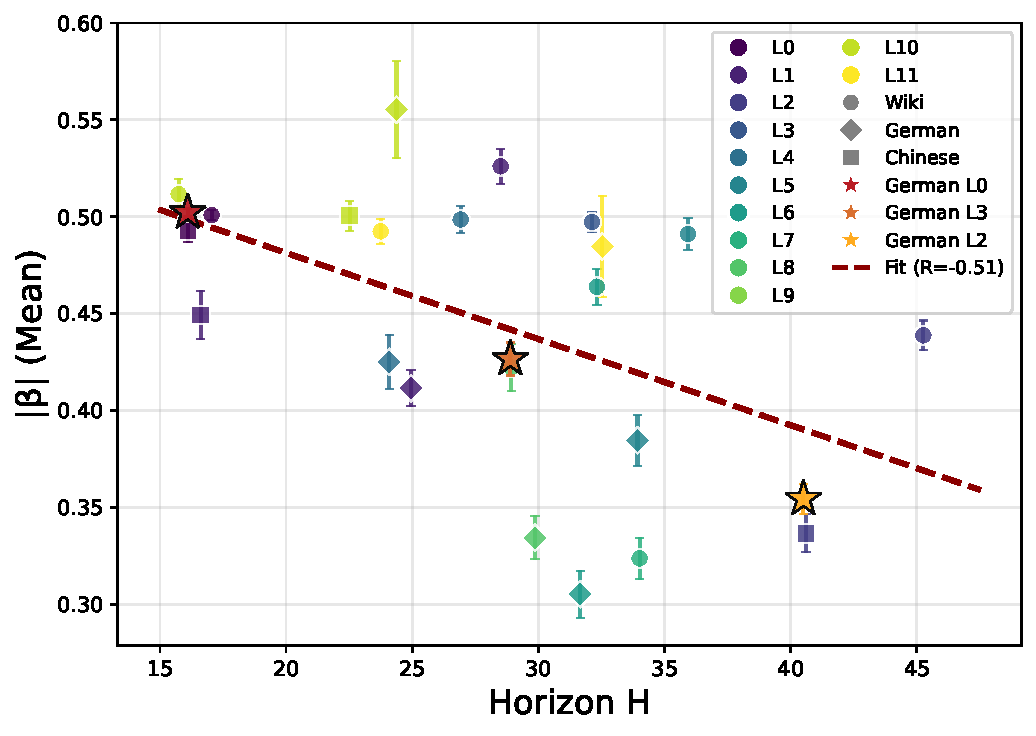
\includegraphics[width=\textwidth]{BERT_slope_vs_H_stars_mean.pdf}
    \caption{Mean error}
\end{subfigure}
\hfill
\begin{subfigure}[b]{0.48\textwidth}
    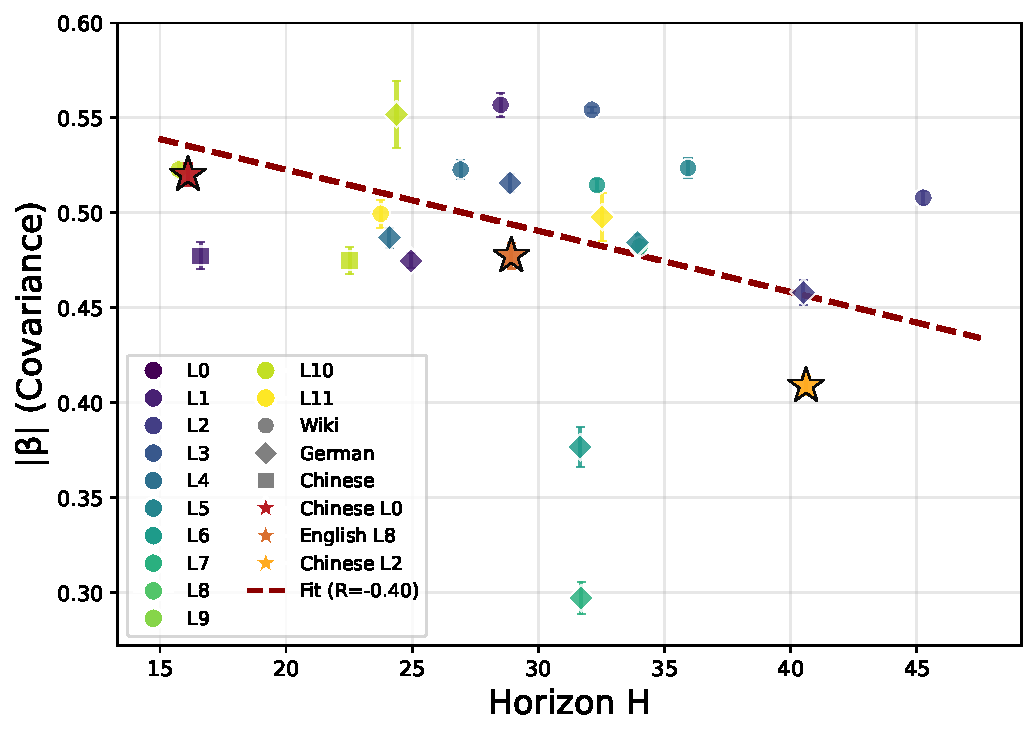
\includegraphics[width=\textwidth]{BERT_slope_vs_H_stars_covariance.pdf}
    \caption{Covariance error}
\end{subfigure}
\caption{\textbf{Convergence rate $|\beta|$ versus horizon $H$ across
  BERT-base-uncased's layers $0$--$11$ and all Wikipedia text distributions.}
  Markers represent $(\text{layer}, \text{text configuration})$ pairs; shapes
  denote text sources (Wikipedia EN/DE/ZH) and colors indicate layers.
  Larger $|\beta|$ implies faster convergence.
  The convergence rate $|\beta|$ is estimated via log-log linear regression of
  the per-token mean (left) or covariance (right) error against $n$, with
  $n \in [1000, 5000]$ i.i.d.\ sampled keys and $k \in [500, 1000]$ Monte Carlo
  repetitions. Star markers denote the configurations whose detailed convergence
  curves are displayed in Figure~\ref{fig:bert_convergence}.
  The dashed line is a linear fit across all points.}
\label{fig:bert_slope}
\end{figure}

\begin{figure}[htbp]
\centering
\begin{subfigure}[b]{0.48\textwidth}
    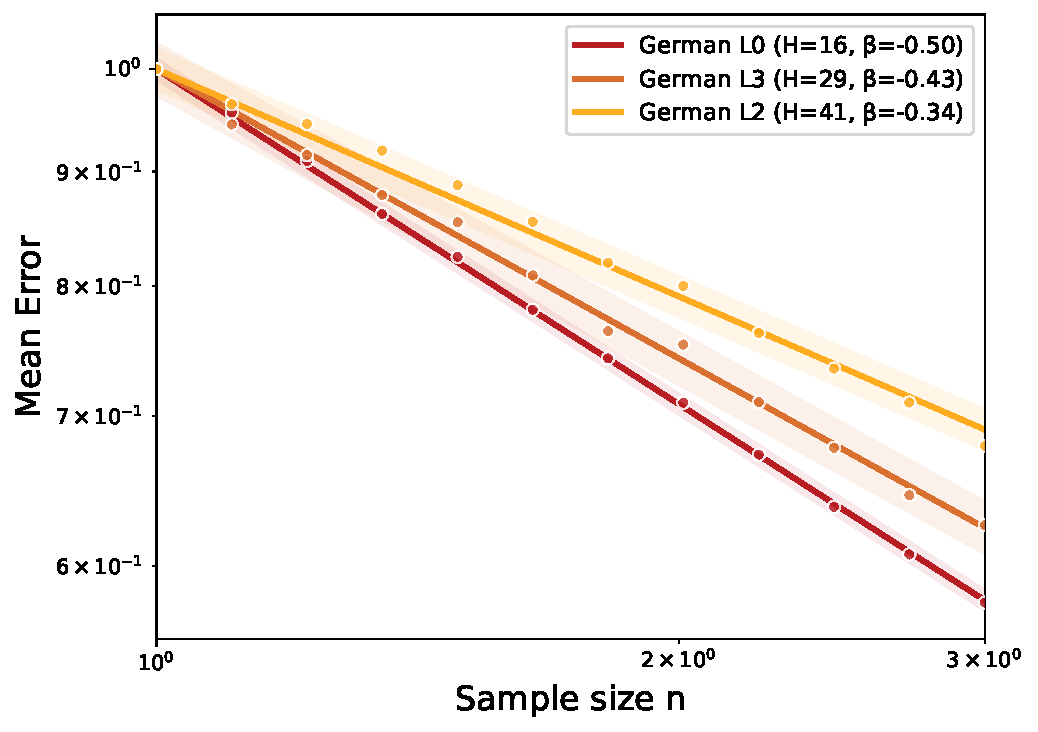
\includegraphics[width=\textwidth]{BERT_convergence_stars_mean.pdf}
    \caption{Mean error}
\end{subfigure}
\hfill
\begin{subfigure}[b]{0.48\textwidth}
    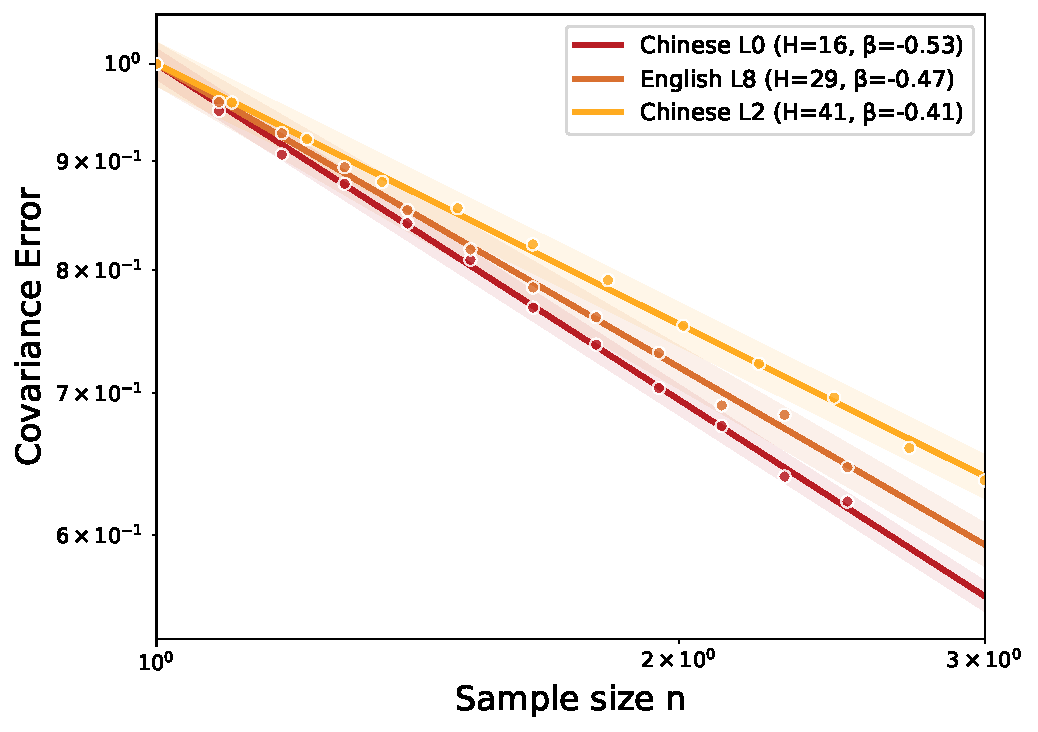
\includegraphics[width=\textwidth]{BERT_convergence_stars_covariance.pdf}
    \caption{Covariance error}
\end{subfigure}
\caption{\textbf{Convergence curves for starred layers.}
  Mean error (left) and covariance error (right) versus subsample size $n$ for
  the three starred configurations from Figure~\ref{fig:bert_slope}, using
  BERT-base-uncased (dense attention).
  Markers show the averaged $\ell_2$ errors over $k=500$--$1000$ subsamples,
  with $\pm 3$ standard-error bands.
  Log--log linear fits yield power-law exponents $|\beta|$ (legend), with error
  scaling as $n^{-|\beta|}$.
  From dark red to light orange as the horizon $H$ increases, confirming the
  slow-down predicted by Theorem~5.3.}
\label{fig:bert_convergence}
\end{figure}

\FloatBarrier

%% ============================================================
%% SECTION 2: Windowed (non-i.i.d.) sampling experiments
%% ============================================================

\section{Windowed sampling experiment}

\begin{figure}[htbp]
\centering
\begin{subfigure}[b]{0.48\textwidth}
    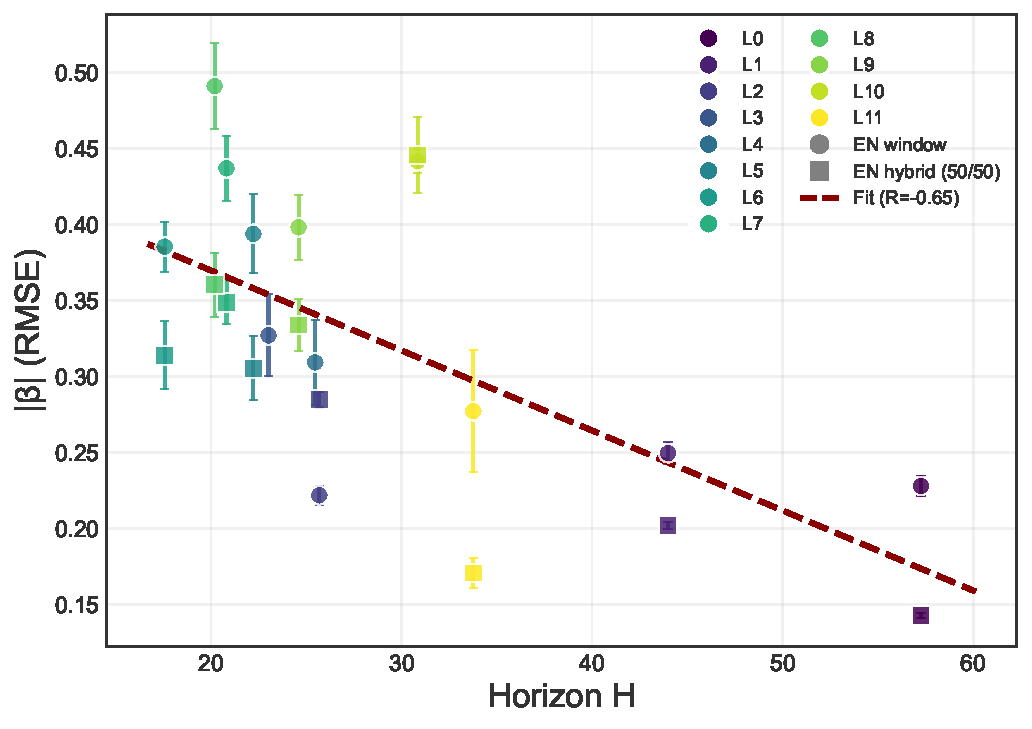
\includegraphics[width=\textwidth]{Window_RMSE_slope_vs_H.pdf}
    \caption{RMSE error}
\end{subfigure}
\hfill
\begin{subfigure}[b]{0.48\textwidth}
    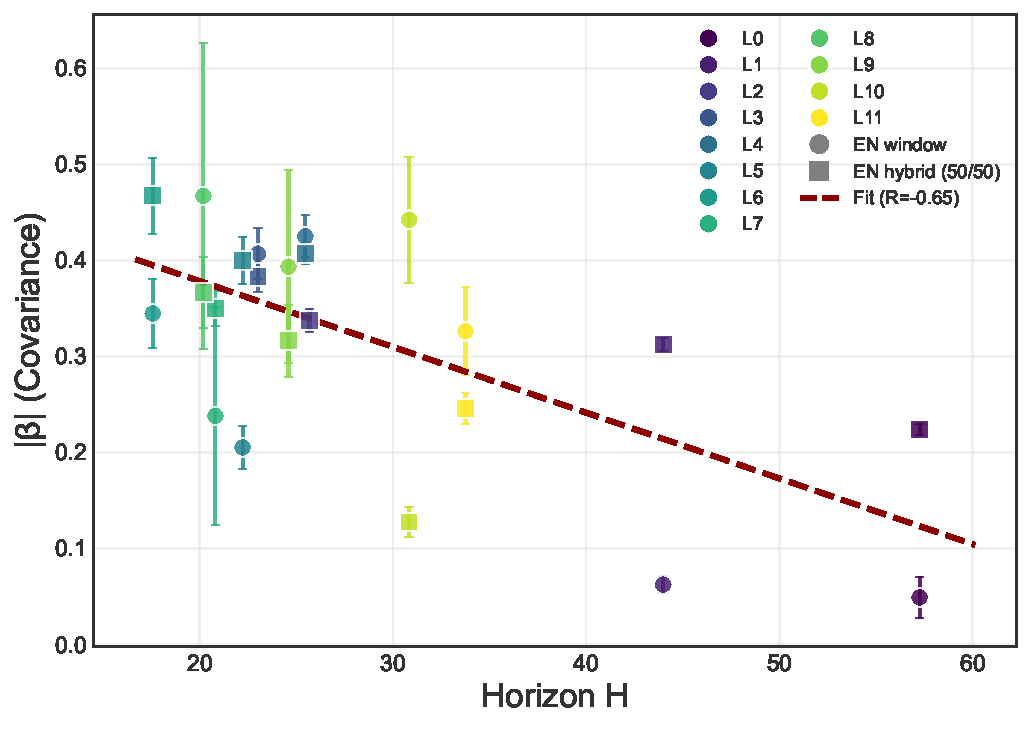
\includegraphics[width=\textwidth]{Window_COV_slope_vs_H.pdf}
    \caption{Covariance error}
\end{subfigure}
\caption{\textbf{Convergence rate $|\beta|$ versus horizon $H$ under non-i.i.d.\
  windowed sampling.}
  BigBird-RoBERTa's layers $0$--$11$ on English Wikipedia, under two sampling
  strategies: fixed-random (EN window, $r=50$ random tokens outside a sliding
  window of size $n-r-1$) and hybrid (EN hybrid 50/50, half window and half
  random tokens). Colors indicate layers. The negative trend (fit slope
  $R=-0.65$) confirms that the slow-down driven by $H$ persists under structured,
  non-i.i.d.\ sampling.}
\label{fig:window}
\end{figure}

\FloatBarrier

%% ============================================================
%% SECTION 3: Uniform distribution on the unit sphere
%% ============================================================

\section{Synthetic experiment: uniform distribution on the unit sphere}

\begin{figure}[htbp]
\centering

\includegraphics[width=0.65\textwidth]{sphere_convergence.pdf}
\caption{\textbf{Convergence rate $|\beta|$ versus horizon $H$ for uniform
  distributions on the unit sphere.}
  Empirical convergence rate exponents $|\beta_{\mathrm{mean}}|$ and
  $|\beta_{\mathrm{cov}}|$ as a function of attention horizon $H$ for token
  embeddings drawn uniformly from the unit sphere $\mathbb{S}^{d-1}$.
  The grey dashed line indicates the classical rate exponent $|\beta_0| = 0.5$
  corresponding to the parametric rate $1/\sqrt{n}$.
  The same slow-down as in the Gaussian case is observed as $H$ increases,
  confirming that the sub-parametric convergence regime predicted by
  Theorem~5.3 extends beyond Gaussian distributions.}
\label{fig:sphere}
\end{figure}

\FloatBarrier

%% ============================================================
%% SECTION 4: Downstream classification experiments
%% ============================================================

\section{Downstream classification experiment}

\begin{figure}[htbp]
\centering
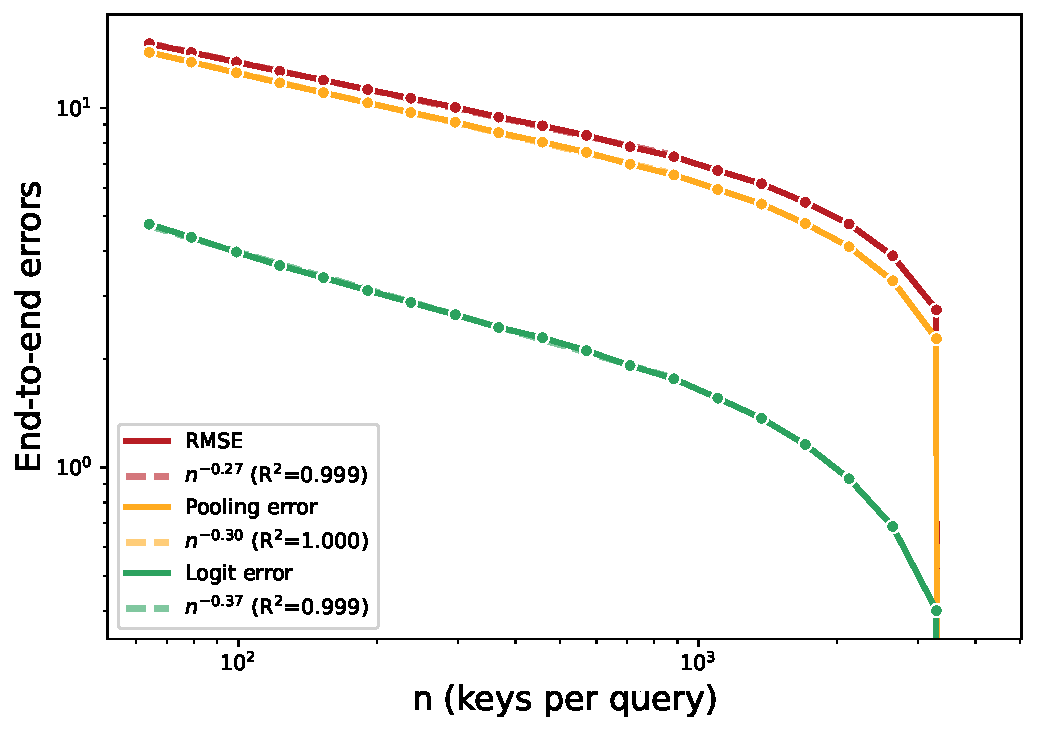
\includegraphics[width=0.65\textwidth]{downstream_task_end_to_end_errors.pdf}
\caption{\textbf{End-to-end error convergence versus number of keys per query $n$.}
  We observe sub-parametric convergence on downstream tasks, with RMSE
  ($\beta=0.27$), pooling error ($\beta=0.30$) and logit error ($\beta=0.37$)
  all scaling as $n^{-\beta}$ with $\beta < \tfrac{1}{2}$, consistent with
  Theorem~5.3. Experiment: BigBird-RoBERTa-base fine-tuned for $3$ epochs with
  mean pooling on arxiv-classification (11 categories, dense accuracy $86.4\%$),
  with $n$ i.i.d.\ sampled keys per query used to compute attention at each layer.
  Dashed lines show power-law fits on $n \leq 884$.}
\label{fig:downstream_end_to_end}
\end{figure}

\begin{figure}[htbp]
\centering
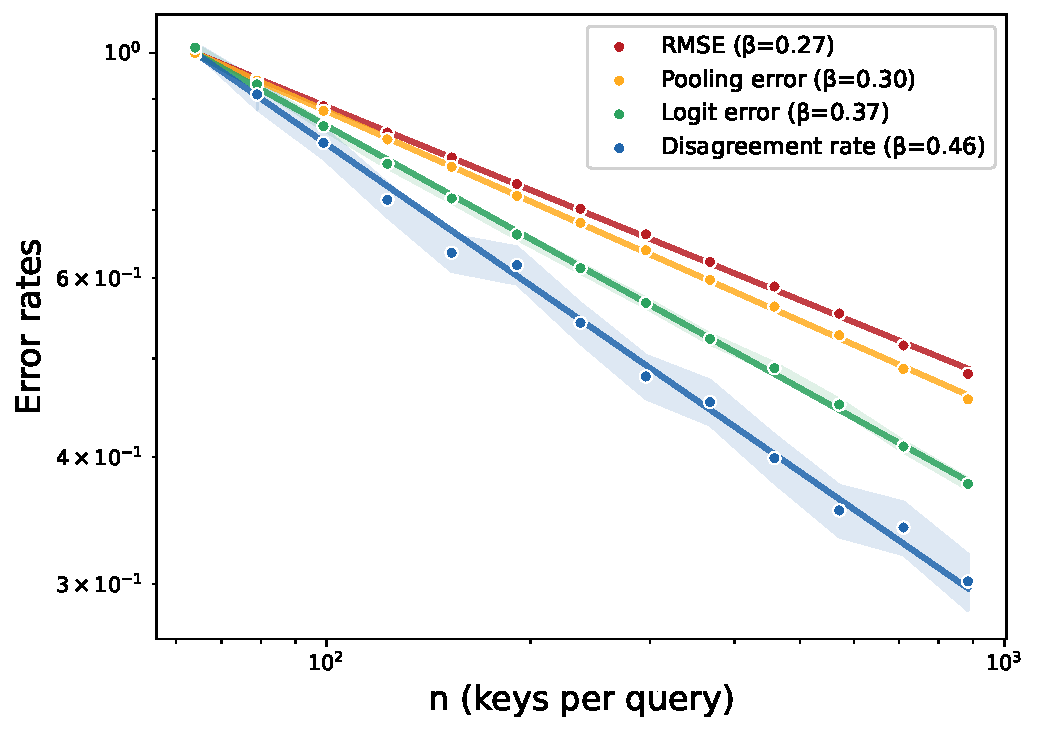
\includegraphics[width=0.65\textwidth]{downstream_task_classification_errors.pdf}
\caption{\textbf{Normalized error rates versus $n$.}
  All downstream error metrics exhibit sub-parametric convergence $n^{-\beta}$
  with $\beta < \tfrac{1}{2}$: RMSE ($\beta=0.27$), pooling error ($\beta=0.30$),
  logit error ($\beta=0.37$) and disagreement rate — fraction of examples where
  sparse and dense predictions differ — ($\beta=0.46$). Downstream metrics
  converge more rapidly than embedding-level metrics. Shaded bands show
  $\pm 3$ standard-error intervals.}
\label{fig:downstream_errors}
\end{figure}

\begin{figure}[htbp]
\centering
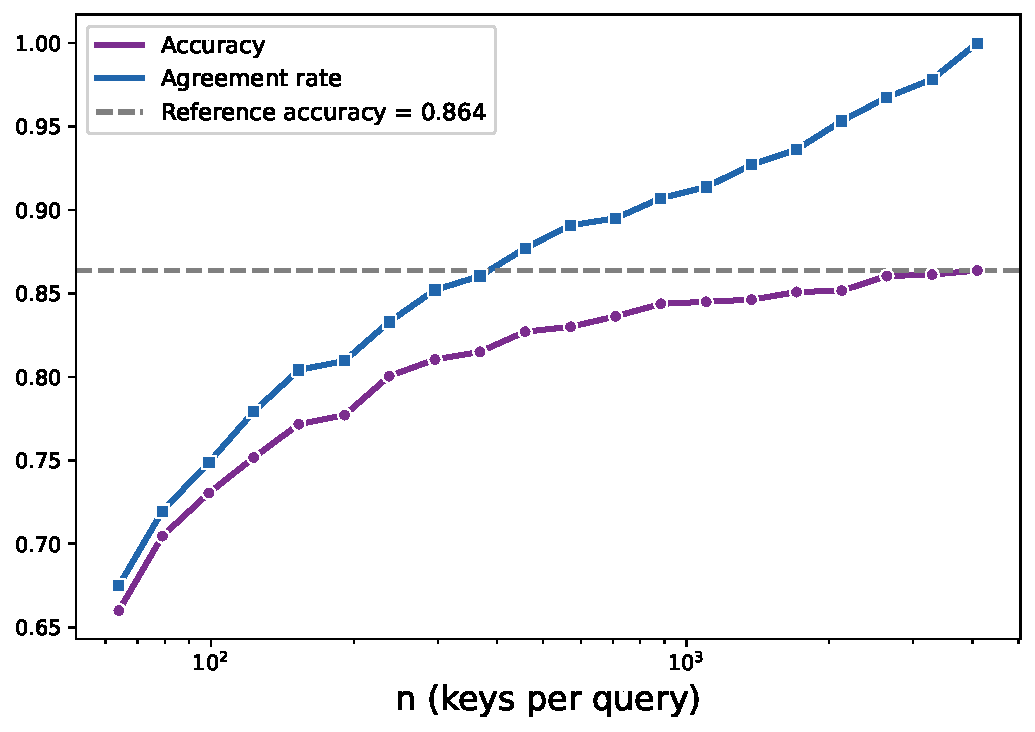
\includegraphics[width=0.65\textwidth]{downstream_task_accuracy_agreement.pdf}
\caption{\textbf{Classification accuracy and agreement rate versus $n$.}
  Accuracy (fraction of correctly classified examples) and agreement rate with
  the dense model (fraction of examples where the sparse and dense models predict
  the same label). The reference accuracy (dashed line) is $86.4\%$. The
  agreement rate converges to $1$ as expected, and the accuracy approaches the
  dense model's performance with diminishing returns: with only $25\%$ of keys
  ($n=1101$ out of $4096$), the model already achieves $84.5\%$ accuracy, and
  doubling the number of keys from $n=1101$ to $n=2124$ yields only a $+0.7\%$
  accuracy gain.}
\label{fig:downstream_accuracy}
\end{figure}

\FloatBarrier

\end{document}